\chapter{Reference management}
\label{sec:literature}

For typesetting our first thes\replaced[id=C]{i}{e}s in \LaTeX{}, the last core functionality to learn is citing literature.
Our references are gathered in a bibliography file.
Once we reference one of its entries from our \LaTeX{} document, Bib\TeX{} (a 
program similar to the standard \acro{PDF}\LaTeX{} compiler)\todo{either adjust 
PdfLaTeX here or in the other locations where it is used, so that it is 
consistent } can insert automatically generated citations.
It will format them in a bibliography style of our choice.

\section{The bibliography file}
Our \textbf{bibliography collection} consists of multiple literature entries in a pre-defined format, such that they can be processed by Bib\TeX{}.
An exemplary item can be seen in \cref{lst:bibfile-sample-entry}.

\begin{figure}[H]
  \begin{minted}[autogobble]{latex}
  @article{turing1990,
    title={The chemical basis of morphogenesis},
    author={Turing, Alan Mathison},
    journal={Bulletin of mathematical biology},
    volume={52},
    pages={153--197},
    year={1990},
    publisher={Springer}
  }
  \end{minted}
  \caption{Exemplary bibliography entry}
  \label{lst:bibfile-sample-entry}
\end{figure}

The type of the bibliography entry is specified after the opening \texttt{@} sign (e.\,g., article, book, proceedings, …).
What follows is a list of important attributes like title and author.
Whether they are required or not depends on the \added[id=C]{type of the }entry\deleted[id=C]{ type}.
In any case, we will need the first entry after the opening braces: the Bib\TeX{} key.
This is the identifier that we will use to reference the entry in our \LaTeX{} document.
Bib\TeX{} keys can be chosen freely, but have to be unique.
Typically, they will consist of a combination of authors, publication dates, and topics.

\textbf{Bibliography files} can be compiled manually, yet it is more common to use programs like JabRef,\footnote{Cf. \url{https://www.jabref.org/}.} Zotero\footnote{Cf. \url{https://www.zotero.org/}.} or the widely-used software Citavi\footnote{Vgl. \url{https://www.citavi.com/de}.}.
While JabRef operates directly on your bibliography file, Zotero and Citavi projects\footnote{Vgl. \url{https://www1.citavi.com/sub/manual5/de/exporting_to_bibtex.html}.} can be exported to bibliography files to use them in \LaTeX{} documents.

\textbf{Bibliography entries} are provided by many academic search engines, including Google Scholar (cf. \cref{fig:google-scholar-bibtex}).
When using them, make sure that the entries are cohesive across your reference collection and complete with regard to their attributes.
A high-quality (although, unfortunately, incomplete) source for Bib\TeX{} entries is the \replaced[id=C]{\acro{DBLP}}{dblp} Computer Science Library.\footnote{Available at \url{https://dblp.org/search}.}

\begin{figure}[H]
  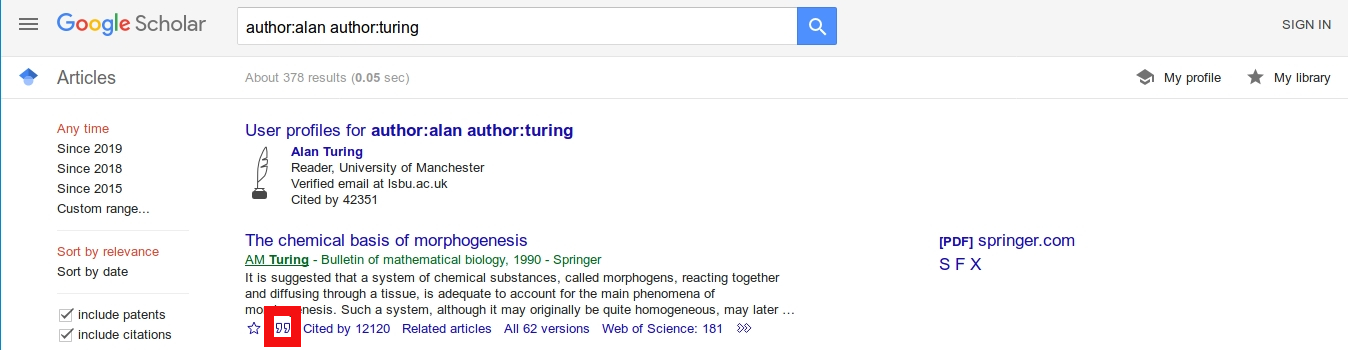
\includegraphics[width=\textwidth]{graphics/google_bibtex1.jpg}  
  
\includegraphics[width=\textwidth]{graphics/google_bibtex2.jpg}  
  \caption{Loading Bib\TeX{} entries from Google Scholar}
  \label{fig:google-scholar-bibtex}
\end{figure}

\section{Citing}
Bib\TeX{} extends \LaTeX{} by several commands (cf. \cref{tbl:bibtex-commands}). 
Make sure to include the \mintinline{sh}{natbib} package for this purpose.

\begin{table}[H]
  \centering
  \begin{tabular}{ll}
  \toprule
  Function                 & Command \\ \midrule
  Citing sources           & \mintinline{latex}{\cite{<source>}} \\
  Citing pages             & \mintinline{latex}{\cite[p. 15]{<source>}} \\
  Custom citations         & \mintinline{latex}{\cite[<prefix>][<suffix>]{<source>}} \\
  Including the bibliography     & \mintinline{latex}{\bibliography{<bibliographyfile>}} \\
  Setting the bibliography style & \mintinline{latex}{\bibliographystyle{<style>}} \\ \bottomrule
  \end{tabular}
  \caption{Commands for citations}
  \label{tbl:bibtex-commands}
\end{table}

The \mintinline{latex}{<source>} of a citation is always a Bib\TeX key.
The list of available citation styles\footnote{Head to Overleaf for a rather complete list: \url{https://www.overleaf.com/learn/latex/Biblatex_citation_styles}} includes alpha, natdin, and apa\todo{Großschreiben oder dicktengleich?}.
The table of references will always appear where the \mintinline{latex}{\bibliography{…}} command was put.
The \mintinline{latex}{\cite} command comes with many variants.\footnote{cf. \url{https://www.economics.utoronto.ca/osborne/latex/BIBTEX.HTM}}

\Example{lst:natdin-example}{literature/natdin-example}{literature/natdin-example_bib}{Exemplary citations in the \mintinline{latex}{natdin} style.}
